%%%%%%%%%%%%%%%%%%%%%%%%%%%%%%%%%%%%%%%%%%%%%%%%%%%%%%%%%
\chapter[Design of the program]{Design of the program}
\label{chap:design_of_the_program}

This chapter focuses on the program's design and thoughts behind it.\\

From the beginning the author knew that he wanted to accomplish three things:
\begin{itemize}
	\item Harvest tweets
	\item Analyze the harvested tweets
	\item Display the results
\end{itemize}

So it naturally made sense to create separate classes for each of those tasks. The author also decided to
create a main class for the program, whose task would be to call the other classes with appropriate parameters
and display the program's status during runtime. Then for the additional feature, to save the tweets collected
in a database, it seemed only natural that the class responsible for the tweet harvesting should be the one that
saves the data and offers other classes access to the data to the database.\\

After looking at a few database solutions the author decided to use the Redis solution because of its simplicity
and ease of use and also to minimize time required for the author to familiarize with the solution since he had
used Redis in a different DTU course this semester.\\

The program therefore consists of four separate Python classes and a Redis database. Each module servers a specific 
purpose in order to accomplish the program's objective. Section 2.4 shows the class overview.

\section{Class FootballAnalyzer} \label{sec:FootballAnalyzerDesign}
The FootballAnalyzer class is the main class in the program and gives other classes the parameters needed 
and receives the data from them. It also displays on the command line the progress of the search, analysis
and html creation. 

\section{Class TwitterAggregator} \label{sec:TwitterAggregatorDesign}
The TwitterAggregator purpose is to search Twitter for tweets, get and save the relevant data to a database
and offer other classes the chance to retrieve the tweet data that has been harvested.

\section{Class SentimentAnalyzer} \label{sec:SentimentAnalyzerDesign}
The SentimentAnalyzer's job is to create a Naive Bayes classifier that uses manually analyzed data, created
by the author, to train how to recognize positive, negative and neutral tweets. The class then takes a list
of tweets and performs a sentiment analysis to classify them into appropriate categories and returns a list
with the classification information appended to the list.

\section{Class HTMLCreator} \label{sec:HTMLCreatorDesign}
The HTMLCreator is the class responsible for creating the web page that displays the results from the football
analyzer. It takes a dictionary of statistics gathered while harvesting and analyzing the tweets and a list of 
all tweets analyzed in the run of the program. \\

The class then displays the statistics, creates a word cloud of the most popular words used in the tweets and
lists every tweet sent to it, colored in a way so that it is easy to see how the classifier classified each
tweet that it was give.

\section{Overview} \label{sec:ClassOverview}
\begin{figure}[ht]
	\centering
		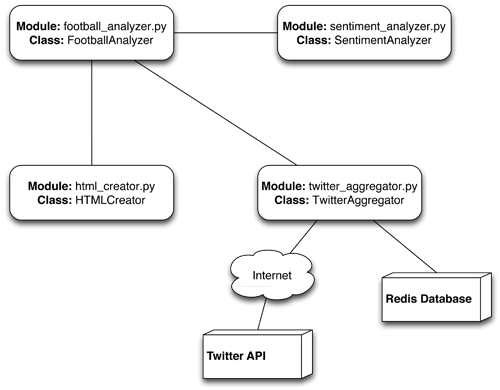
\includegraphics[height=330px]{images/ClassOverview.png}
	\caption{ Class overview of the football analyzer }
	\label{fig:images_ClassOverview}
\end{figure}